\subsection{Data for help tests}
\subsubsection{Goal 1}
Goal 1 is "The individual could allow (or refuse) Data4Help to use their data".

\begin{figure}[H]
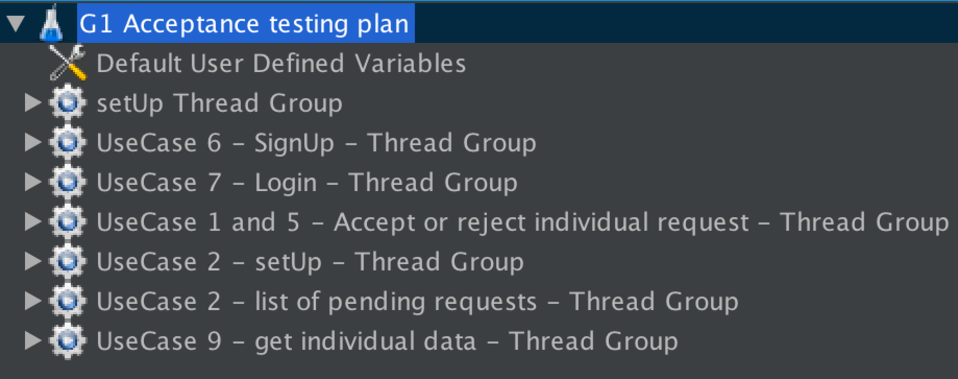
\includegraphics[width=0.7\linewidth]{images/goal1}
\centering
\caption{ JMeter G1 Acceptance Testing }
\label{fig:goal1}
\end{figure}

The uses cases that concerns G1 are: UC1, UC2, UC3, UC4, UC5, UC6, UC7 and UC9. These have been retrieved by looking
at the requirement traceability matrix in the RASD.  

\begin{itemize}
\item 
UC1 regards the scenario in which a user accepts or refuses a request. \\
The successful case has been tested (no exception is present) by using some requirements that involves the
third party registration and the possibility to send individual request. In particular, after having created a new third party customer,
and a new user; a request from that customer to the user is made. The user retrieves the list of pending requests (that contains only that
element) and approves/rejects it.

\item 
UC2 involves the fact that a logged individual can access his pending requests. \\
For testing it, a great number of third party customers has been registered: they all send a request to the same user.
The user retrieves all the pending requests and a check on the number of pending request: the behaviour is correct.
The exceptional case, requires the use of the front end: in particular, it is said that if no pending requests are available, then a message
should been shown to the user: however, no message is displayed.

\item 
UC3 and UC4 regards sending notification to the third party when a user approve or reject an individual request. By recording the HTTP Request after changing a request to approved or rejected, this does not invoke any HTTP request. Therefore, we suppose that they are not working properly and because it cannot be further tested.

\item 
UC5 regards the acceptance and the refusing of requests. In particular, they are similar to UC1, except for the fact
that they are analyzed from a third party customer point of view. For this reason, they have been tested together with UC1. 
In particular, after that the request is approved, we have checked that in the subscriptions
of the third party there exists one on a SSN that is equal to the user that accepted the request.

\item UC6 involves the sign up of users and third parties. The successful case has been tested and also the exception cases in which SSN, email and taxCode
are already present in the system. \\
The result is the following: userId and accessToken returned by the server are correct. In particular, they have been used to check
if the user was registered by performing an HTTP request to retrieve the user's information.  \\
The exception about checking if fields are empty or not has been checked with manual testing since this is something that is implemented in the front
end.

\item UC7 consists in logging users and third parties into the system. The normal event flow and the cases of wrong credential has been
tested.
The same check adopted in UC6 has been used here. \\ 
The exception that involves missing password or email, has been checked with manual testing since this is something that is implemented in the front 
end.

\item UC9 regards the access to individual data. This test has also been done with JMeter using third parties and individuals which are generated from the folder src/seeders created by the other team. In particular the Delta Dore Italia third party has been used to access individual data regarding the user Andrea Esposito. Since data are autogenerated, we do not know how many data it has, but generally,after starting the server it should immediately send a data of Andrea Esposito, therefore in the test we check if it exists at least one data.

\end{itemize}


\subsubsection{Goal 2}
Goal 2 is : "the third-party company should be able to access data of a specific individual".

\begin{figure}[H]
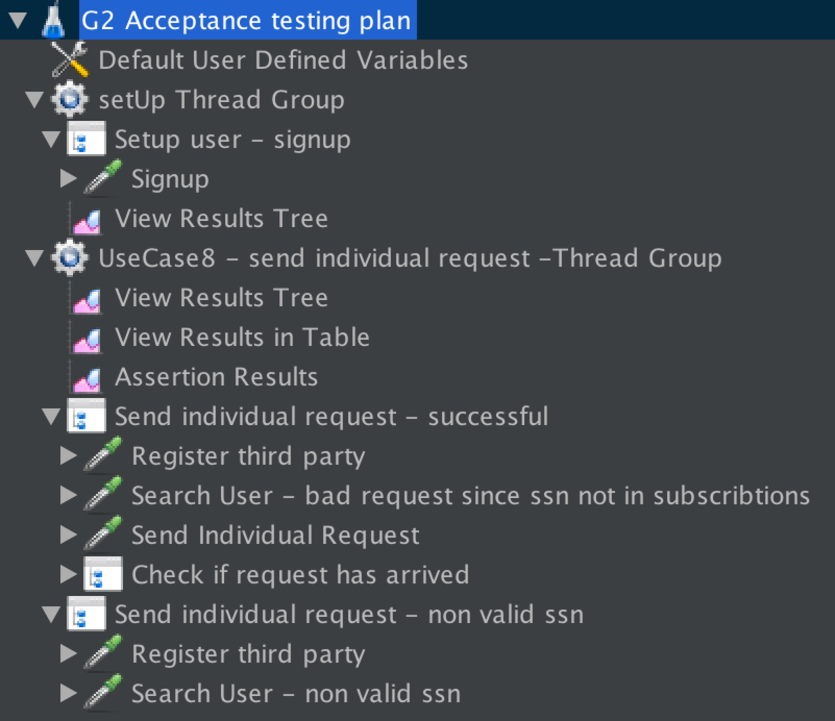
\includegraphics[width=0.7\linewidth]{images/goal2}
\centering
\caption{ JMeter G2 Acceptance Testing }
\label{fig:goal2}
\end{figure}

The uses cases that regards G2 are: UC6, UC7, UC8, UC9, UC32 and UC33.  

\begin{itemize}
\item UC6, UC7 and UC9 were already presented above, while discussing G1.

\item UC8 analyses the case in which a third party sends a request. \\
To test it, basically, the idea is searching for the user SSN. 
If it is found, it returns a bad request (i.e. this seems strange, but it is the correct chain-flow) with a specific message "Should send a
request to the individual to access his data". This happens because the third party customer is not subscribed to the data of that user, and
therefore a request has to be sent.
Thus, after that, it is possible to send a request: to check if things work properly, we have to be sure that the user has received a new pending request. In the end  the result is correct and the exceptions have been tested successfully. 

\item UC32 and UC33 regards the receive of notification of approved/rejected individual requests by third party or AutomatedSOS. For the same reason of UC3 and UC4, they are not working properly for us since not testable.

\end{itemize}

\subsubsection{Goal 3}
Goal 3 is "the third-party company should be able to access anonymized data of groups
of individuals under certain constraints".

\begin{figure}[H]
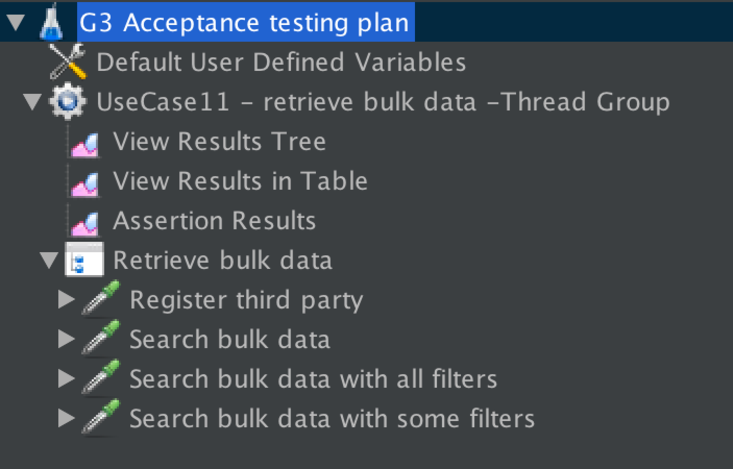
\includegraphics[width=0.7\linewidth]{images/goal3}
\centering
\caption{ JMeter G3 Acceptance Testing }
\label{fig:goal3}
\end{figure}

The uses cases that involves G3 are: UC6, UC7, UC11 and UC12.  

\begin{itemize}
\item 
As already mentioned, the first two use cases are already tested above during the test of G1.

\item 
UC11 and UC12 regards the access to bulk data.
During the test of UC11 and UC12, it is impossible to understand when there is an error message. 
In fact by doing the manual test, even 3 blocks of anonymized data are returned and no error message is shown. 
This is in conflict with what is expressed in the description of the use case of the RASD document. 
Indeed, it is mentioned that "if there are less than 1000 individuals in the request of data, an error is returned":
however, this does not happen. \\
To test the normal flow, however, one should note that to have many data into the system, it is necessary to leave the server up: the more the
time passes, the more the pieces of data available. In UC11, we test the response code of the HTTP request to access the bulk data: the
behaviour is correct. This is due to the fact that there is no possibility of inserting data, and, therefore, it is not possible to know which
and how many pieces of data are available, in order to do more specific controls. 

\end{itemize}

\subsubsection{Goal 4}
Goal 4 is "the third-party company could subscribe to get new data related to specific
individuals or previously saved search".

\begin{figure}[H]
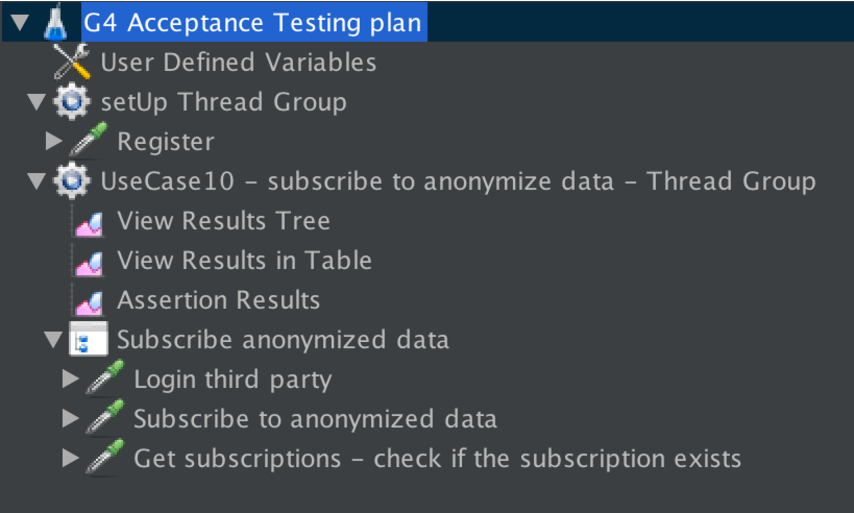
\includegraphics[width=0.7\linewidth]{images/goal4}
\centering
\caption{ JMeter G4 Acceptance Testing }
\label{fig:goal4}
\end{figure}

The uses cases that concerns G4 are: UC6, UC7, UC9, UC10, UC11, UC12, UC32, UC33 and UC34. \\

\begin{itemize}
\item 
UC6, UC7, UC9, UC11, UC12, UC33, UC32 are already discussed above

\item 
UC10 consists in the subscription of a third party customer to new user data. \\
In the website, the subscribe is done when a checkbox is crossed during the search of bulk data. 
While testing with JMeter, the search has been skipped and only an HTTP request to directly subscribe has been done.
To check if things work properly, the subscriptions of that third party are retrieved: since the subscription id is present, the
result is correct.

\item 
UC31 regards the send of individual data to third parties subscribed. This process has been discovered during the capture of HTTP Request by using JMeter. Therefore, we suppose that UC31 is working properly since other testing cannot be done due to random generation of data.

\end{itemize}

\subsubsection{Other tests}
As already mentioned, some other tests have been done, manual, by exploring the UI. \\

\par
Indeed, once the application is installed, it is possible to test the correct functioning of the graphic interface. 
The site appears to be well structured in its parts and graphically pleasing. 
The test has found some graphic bugs that do not affect the correct achievement of goals. 
The operations that a user can do on the site are all fairly clear and easy to understand, sign of a correct structuring of the user
interface.
The only operation not explained is the registration of the third party, where it is required to enter a certificate, without explaining what
it is. Another problem is when a user try to sign up with an e-mail that already exists into the system: an appropriate error message is not shown. (see the figure \ref{fig:bugobject})\\

\begin{figure}[H]
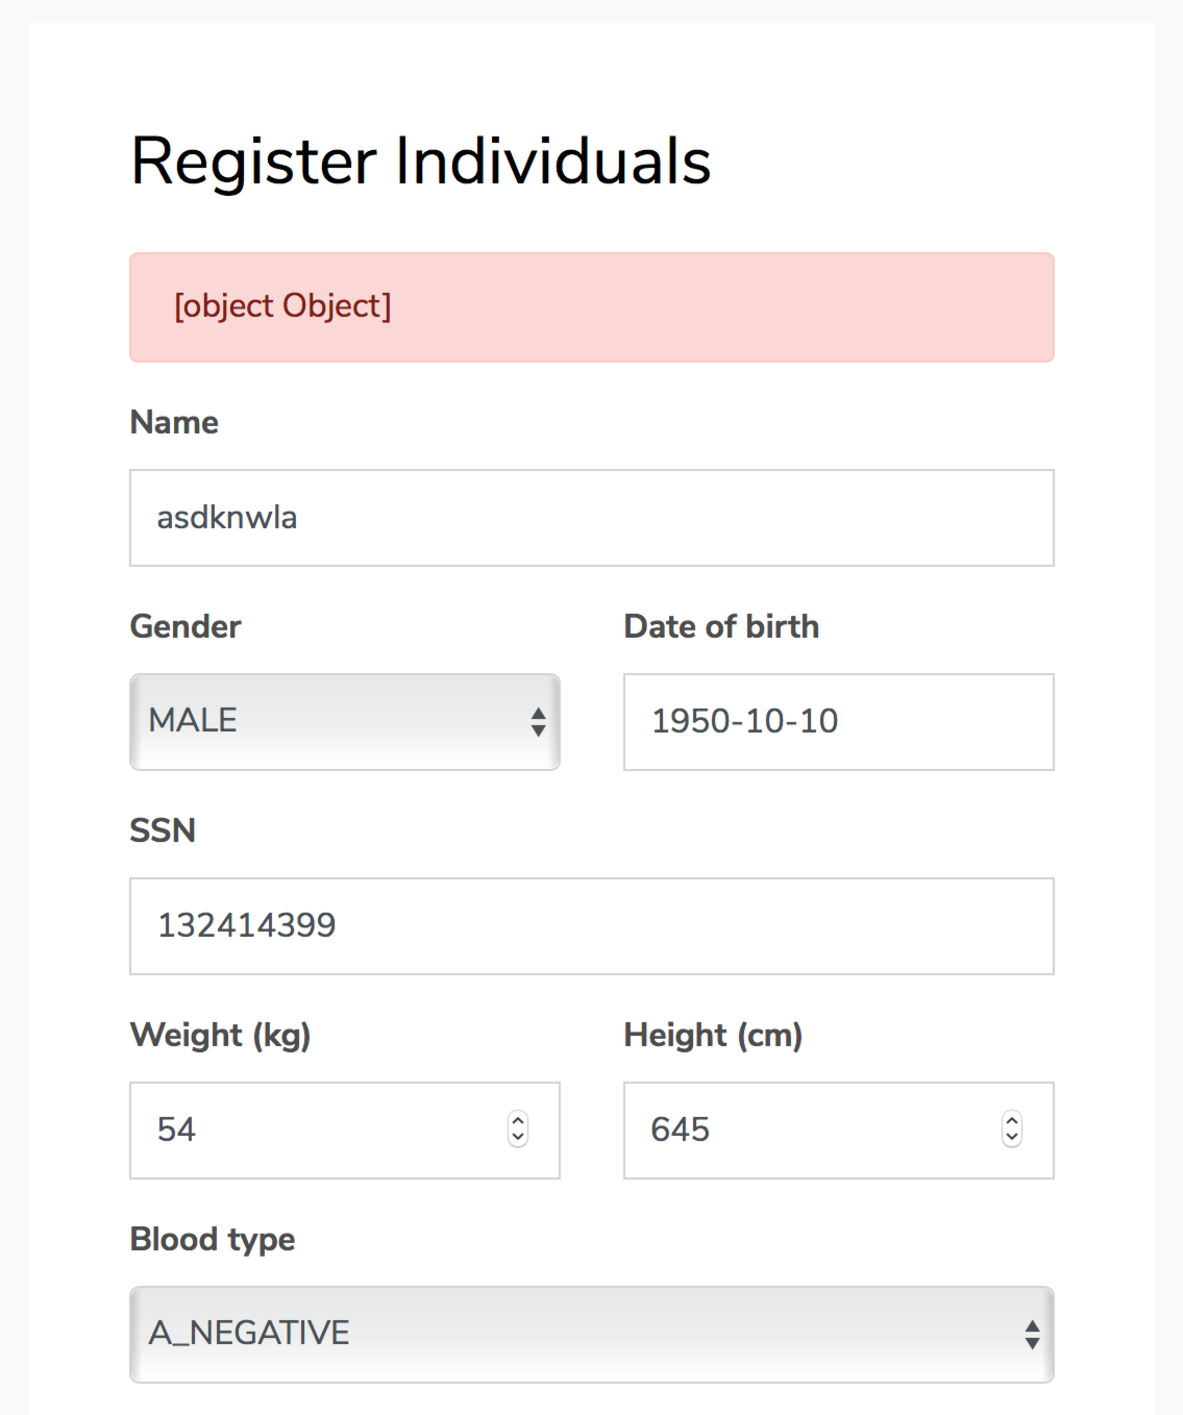
\includegraphics[width=0.7\linewidth]{images/objectError}
\centering
\caption{ UI Bug: [object Object] }
\label{fig:bugobject}
\end{figure}

We have also performed some tests that regards the registration of third party customer, that sends to the users previously
created individual requests and group requests. Finally, back to the user profiles, we have checked that the requests have arrived and that
the user can refuse or accept the requests received.\\

\par
Other than UI tests, we have also performed a test to check if the public API of an individual can be accessed with the userId and accessToken of a third party and viceversa. Indeed, this operation cannot be done and a error message is returned: "The current user is not authorized to perform the operation" (this test is present in OtherTest.jmx of JMeter).

\begin{figure}[H]
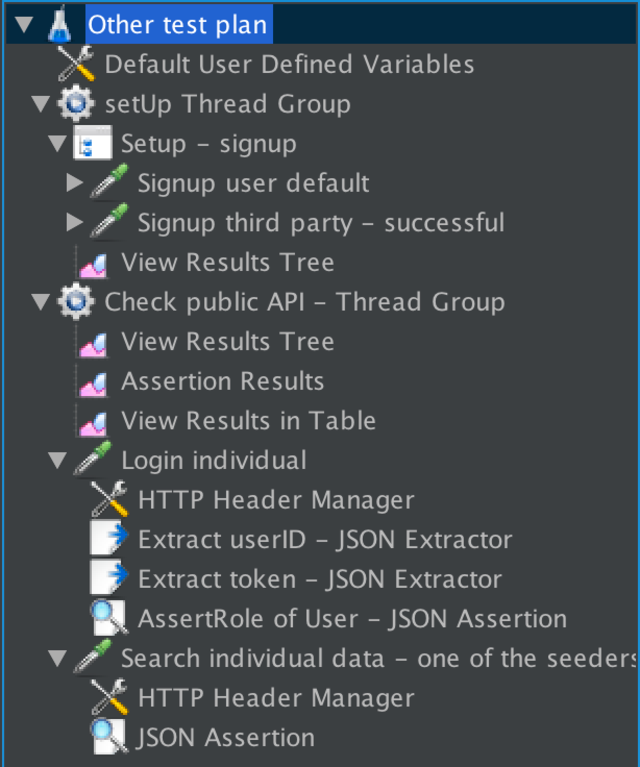
\includegraphics[width=0.7\linewidth]{images/otherTest}
\centering
\caption{ JMeter Other Tests }
\label{fig:othertest}
\end{figure}
